\section{Arbeitskultur}
	\subsection{Einleitung}
Reinhard Kößler definiert den Begriff der Arbeitskultur im ``Lexikon zur Sozialogie`` von Wernern Fuchs-Heinritz als Verschiedenheit von Visionen des Arbeitsverhaltens in Form von Lebensformen, Einstellungen und Reaktionen auf die Anforderungen der Arbeit in industriell-kapitalistischen Gesellschaft. \cite{Fuchs-HeinritzLautmannRammstedtWienold1994}.
Arbeitskultur ist in der ersten Linie eine Teilmenge der Kultur (Sitten, Bräuche, Mentalität usw.) einer Nation. Gemäß dem Carsten Weigelt bedeutet die Arbeitskultur für die jungere Generation - sogenannten ``Digital Natives`` viel mehr als Geld und Karriere. Unter Arbeitskultur wird von ihnen das Wohl im Privatleben und am Arbeitsplatz verstanden.\\ Die Arbeitskultur gehört zum Beratungsprozess und spielt dabei nicht die unwesentlichste Rolle. Welche Arbeitskultur gehört zum Beruf des IT-Beraters? Denn ein IT-Berater ist immer in der Bewegung und Arbeitsplatz ist nicht nur im Büro sondern auch im Zug, im Restaurant oder im Auto. Das ist sehr ersichtlich, dass die Arbeitskultur des Beraters mit der Arbeitskultur den 
Kunden des Beraters unzertrennlich ist. IT-Consultans kennen innerhalb der wenigsten Zeit sehr viele Firmen und deren Mitarbeiter kennen. Berater arbeiten fast die ganze Zeit durch Iteration mit Menschen aus:\\
\\
1) unterschiedlichen Unternehmensebenen (mit unterschiedlichen Arbeitskulturen) angefangen von normalen Mitarbeiter(Interaktion mit Beratern während den Schulungsmaßnahmen bei IT-Neueinführung) bis zu Top-Managementebenen(Interaktion mit Beratern während den strategischen Fragen wie Analyse von Geschäftsprozessen mit folgender Einführung von Anwendungssoftware ) \\
\\
2) verschiedenen Branchen (mit verschiedenen Arbeitskulturen) wie Finanzdienstleistung,Fahrzeugbau, Großhandel usw. (sieh Abb. 4.2)\\
\begin{figure}[ht]
\centering
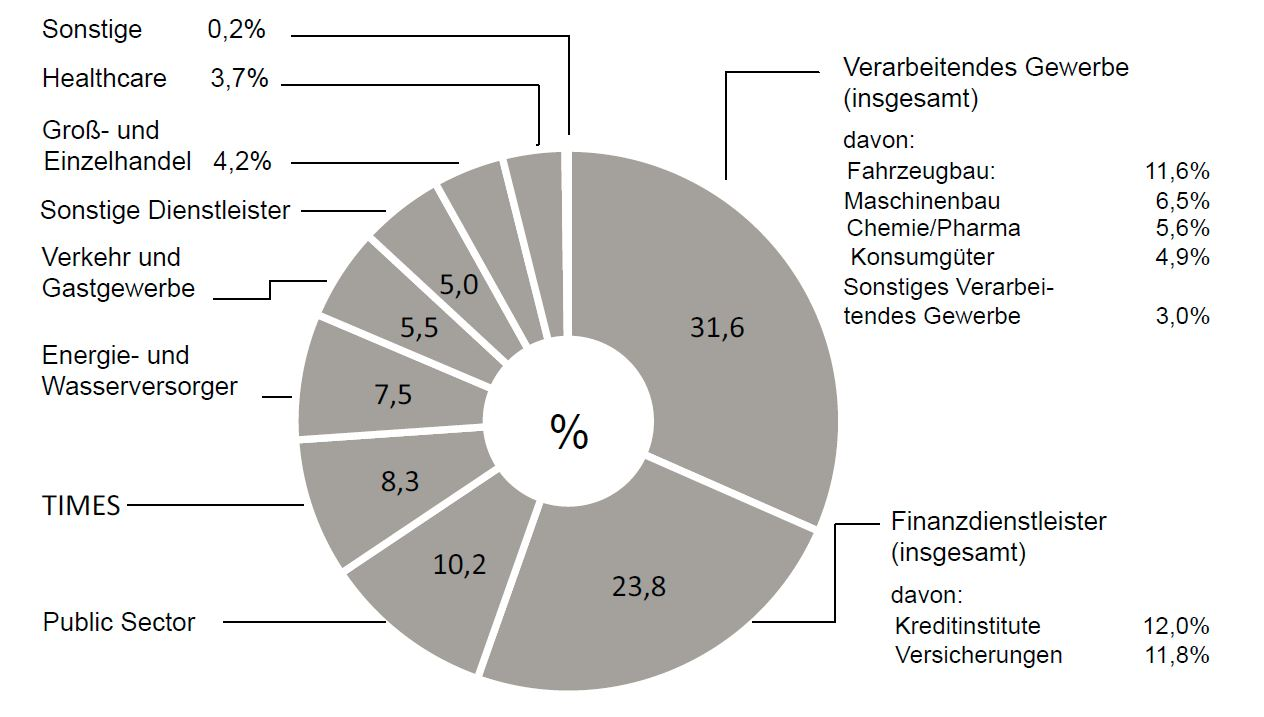
\includegraphics[width=10 cm]{./images/Auft_U_Beratung}
\caption{Aufteilung Unternehmensberatungen nach Branchen}
\label{fig:AufteilungUnternehmensberatung}
\end{figure}
\\
	3) unterschiedlichen Länder mit jeweils einzigartigen Kulturen sowie Arbeitskulturen.\\
	 In diesem Punkt werden 2 Standardfälle erklärt, um die Bedeutung der Arbeitskultur im Beratungsprozess näher zu erläutern.\\
	 \\
	 a) Das 1. Fall ist ein IT-Consulting-Unternehmen mit eingestellten Beratern, die aus unterschiedlichen Ländern kommen, unterschiedliche Sprache sprechen und sich kulturell enorm unterscheiden. Wichtig für die Arbeitskultur an dieser Stelle ist kulturellen Gleichgewicht herzustellen und dauerhaft zu behalten. Diese Berater arbeiten zielgerichtet und ständig im Team. In diesem Fall wird dem Author dieser Arbeit sehr interessant, inwieweit sich kulturelle Unterschiede auf das gemeinsame Ziel des Beratungsprozesses bei der Softwareeinführung auswirken können. Auch interessant ist hier wie die IT-Berater aus unterschiedlichen Länder mit Kunden aus Deutschland umgehen, ob die kulturelle Unterschiede einen Einfluss auf Kundenbeziehungen haben oder nicht. \\
	 \\
	 b) Das 2. Fall bezieht sich auf ein deutsches Unternehmen, das sich international agiert und Kunden aus unterschiedlichen Länder betreut. In diesem Fall müssen sich deutsche Mitarbeiter auf unterschiedliche Arbeitskulturen anpassen. Denn ein Meeting während des Mittagsessen in Japan ist widersinnig und wirkt unseriös (in Japan hat das Essen einen unverletzlichen Status), in USA dagegen ist es nicht ungewöhnlich, dass beim Essen wichtige Entscheidungen kollaborativ getroffen werden.\\
	Wegen der zeitlichen sowie thematischen Begrenzung liegt der Autor dieser Arbeit den Fokus nicht auf die Differenzierung dieser zwei Fälle sowie kulturelle Unterschiede der Berater, sondern nur auf die unterschiedliche Arbeitskulturaspekte, die für den Beratungsprozess ausschlaggebend sind. Teilaspekte der Arbeitskultur, die den Autoren dieser Arbeit interessant erscheinen, werden in folgenden Kapiteln vorgestellt und verglichen. In diesem Sinne werden diese zwei Fälle nicht unterschiedlich und nur im Hintergrund behandelt.\\
	\\
\textbf{Das Wesen des IT-Consultings}\\ \\
	Nachdem ich die Arbeitskultur erklärt habe, muss ich das Wesen des IT-Consultings detailierter betrachten. An dieser Stelle ist es unveräußerlich den Beratungsprozess exemplarisch zu zeigen, um die Feinheiten des Prozesses zu verstehen, die von der Arbeitskultur beeinflusst werden.
	IT-Consulting ist eine wichtige Art des Consultings in IT-Fragen eines Unternehmens. Das Wesen des Consultings besteht im Allgemeinen darin, Unternehmen bei der Neustrukturierung des Anwendungslandschaften oder bei der Pflegung der bestehenden Informationssysteme zu unterstützen. Während des gesamten Beratungsprozesses bleibt Berater als externe Experte solange im Unternehmen bis die Probleme, die er mit seinem technischen Fachwissen zu lösen hat, nicht mehr existieren oder selbständig von den Mitarbeitern des Unternehmens gelöst werden können.\\
	Um den Beratungsprozess zu verdeutlichen wird jetzt ein Beispielprozess aus der Praxis der IT-Beratung beschrieben. Ein Online-Handelsunternehmen möchte ein BI-Standardsoftware einführen und die Daten für Analysezwecke aus dem bestehenden ERP-System zu laden, um die potentiellen Kündiger zu vermeiden oder neue Kunden zu gewinnen. Am Anfang jedes Prozesses muss dem Berater die Organisationsstruktur und die Geschäftsprozessabläufe des Unternehmens klar sein, um eine passende Lösung zu finden. IT-Berater haben eine Standardsoftware im Einsatz, um geschäftlichen Probleme eines Unternehmens mit Hilfe von Informationstechnologie zu lösen. Es gibt aber keine Standardlösung die für alle Unternehmensstrukturen passend ist, weil die Unternehmensstrukturen selbstverständlich heterogen sind. Nach dem erfolgreichen Vertragsabschluss zwischen Unternehmen und dem Consultingbetieb beginnt die Analysephase des Beratungsprozesses. Hier wird die Unternehmensstruktur des Online-Handelsunternehmen auseinandergenommen, bis man erkennt wo die Software eingesetzt wird, Stellen wo die Reibungen entstehen werden, welche Ressourcen stehen zur Verfügung und welches Informationssystem sich am besten dafür eignet. Es muss ständig ein Feedback zwischen dem Berater und Unternehmensführer durchführbar sein.\\
	Jetzt wird der Ablauf des Beratungsprozesses intensiver beschrieben. Nach der Analysephase beginnt man der Konzepterstellung indem die Ideen und Pläne in Erfüllung gehen. In der Folge beginnt die Umsetzungsphase,dadurch eine neue IT-Architektur aufgebaut oder die vorhandene ergänzt wird. Im unseren Beispiel wird die ERP-Lösung mit der BI-Lösung erweitert, die vorhandene Architektur bleibt erhalten. In dieser Phase können auch die andere Berater aufgerufen werden, falls es viele komplizierte Realisierungsmaßnahmen gibt.
	Nachdem das Informationssystem erfolgreich in die Unternehmensstruktur integriert ist, beginnen die Schulungsmaßnahmen, damit die Mitarbeiter des Unternehmen in der Lage sind mit diesem System umgehen zu können. Zum Schluss kommt die Wartungsphase und Intensität der Beratungsdienstleistung nimmt langsam ab. Diese Prozesskette kann auch in Form eines Lebenszyklus oder auf der Sprache der Informatik als Endlosschleife  stattfinden.\\
	Diesen Ablauf kann man graphisch am folgenden Modell des ganzheitlichen Beratungsprozesses erkennen(seih Abb. 4.3). Dieses Modell liefert uns die einzelnen Phasen der Beratungsdienstleistung eines Freelancers im Gebiet der Managementberatung. 
\begin{figure}[htp]
\centering
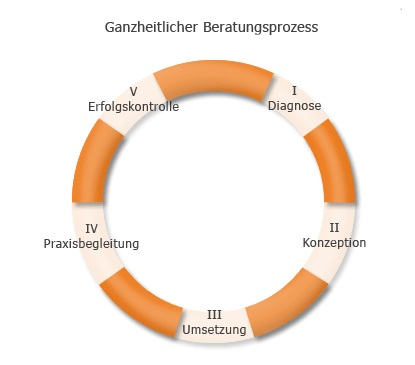
\includegraphics[width=0.7\linewidth]{./images/beratungsproz}
\caption{Phasen des Beratungsprozesses  eines Managementberaters, \cite{PhasenBeratungsprozess} }
\label{fig:beratungsproz}
\end{figure}
	
	\textbf{ Bedeutung der Arbeitskultur für IT-Consulting}\\ \\
	In wie weit ist es wichtig Arbeitskultur für den Beratungsprozess zu betrachten? Anhand vom unseren Beispiel ist es zu erkennen, dass die IT-Berater in jeder Phase der Softwareeinführung mit den Unternehmensvertretern kommunizieren sollen. Es ist wichtig, dass die Berater genug technisches Know-how mitbringen, noch wichtiger sind die Soft Skills, die für erfolgreiche Geschäftsbeziehungen entscheidend sind. ``IT Business is People's Business.`` Damit wird gemeint, dass der Erfolg von   IT-Projekten sowohl auch von den vertrauensvollen Verhandlungen maßgeblich von der Kompetenz des Beraters abhängt. \cite{ITConsRu}
	Welche Social Skills des IT-Beraters sind für Deutscher als obligatorisch herausgestuft? Sind diese persönlichen Eigenschaften auch für die anderen Nationen von der Bedeutung? Unternehmensführung und IT-Berater müssen bei der Lösung des Problems einig werden. Der Berater muss ein Unternehmen für seine vorgeschlagene Lösung überzeugen. Muss man, um dies zu realisieren nur eine gute Software anbieten und als vertrauenswürdiges Unternehmen am Markt agieren oder reichen diese Bedingungen beispielsweise in Indien nicht aus, weil der Berater aus anderer Kaste ist. Denn die Kastenzugehörigkeit hat in Indien bis heute kulturelle und soziale Auswirkungen auf viele Lebensbereiche \cite{KastensystemInd}.
	Für diese Arbeit ist wichtig zu wissen wie die Arbeitskultur in ausgewählten Länder sich unterscheidet und in wie weit diese den Beratungsprozess beeinflussen kann.
	In den folgenden Kapiteln wird Arbeitskultur von ausgewählten Länder(Russland, USA, Deutschland usw.) untersucht und zum Schluss werden einige interessante Fakten verglichen und diskutiert. 
\subsection{Teilaspekte}
	Hier werden Teilaspekte aufgelistet, die für Arbeitskultur von Bedeutung sind (Arbeitsplatz, Mitarbeiterverhältnisse, Hierarchien, Organisation, Lebensumstände etc.).
	Es wurden sich hierfür einige Teilaspekte der Arbeitskultur sowie die zugehörigen Länder durch Brainstorming überlegt. Dazu wird der Übersicht halber eine Matrix aufgestellt. Felder dieser Matrix bleiben zuerst leer und nach dem die einzelne Aspekte von den Ländern recherchiert und vorgestellt werden, wird die Matrix noch mal mit den ausgearbeiteten Feldern ausgefüllt. Damit kann man auch die Rechercheergebnisse testen, ob sie erfolgreich waren oder nicht.\\

\begin{table}[htp]
\begin{tabular}{|c|c|c|c|c|c|c|}
\hline  Aspekt/Land& Deutschland & USA & Russland & Japan & Indien & Brasilien \\ 
\hline 	Hierarchien  & ? & ? & ? & ? & ? & ? \\ 
\hline  Kundenverhältnisse& ? & ? & ? & ? & ? & ? \\ 
\hline  spezielle Rechtslage& ? & ? & ? & ? & ? & ? \\ 
\hline  Grad des intuitiven Handelns& ? & ? & ? & ? & ? & ? \\ 
\hline  Kritikfähigkeit& ? & ? & ? & ? & ? & ? \\ 
\hline  Tagesrythmus& ? & ? & ? & ? & ? & ? \\ 
\hline  Organisation& ? & ? & ? & ? & ? & ? \\ 
\hline  Lebensumstände& ? & ? & ? & ? & ? & ? \\ 
\hline  Zeitmanagement& ? & ? & ? & ? & ? & ? \\ 
\hline  Work-Life-Balance& ? & ? & ? & ? & ? & ? \\ 
\hline 
\end{tabular} 
\caption{Matrix der Arbeitskultur, Quelle: eigene Darstellung xD}
\end{table}
\newpage
%Morgen Hier Kontrolle Weiter
	\subsubsection{Russland}
	Russland ist ein Wachstumsmarkt mit Zukunft. Laut Holger Hirsch ist heute der von damals geschützte russische Markt offen für Exporte und Investitionen aus Deutschland. Dies gilt sowohl für IT-Beratungs Unternehmen, die ihre Softwareprodukte in Russland integrieren auch für russische Manager, die bei der Informationstechnologie auf westliches Know-how setzen.\cite{ITConsRu}\\
	Da der Markt für IT-Beratung neu ist, muss man als IT-Berater aus Westen ganz viele Entscheidungen intuitiv treffen. Hier weden natürlich die Softskills des Beraters gefragt. Technische Fähigkeiten, funktionales Wissen und Branchen-Know-how sind selbstverständlich vorausgesetzt. Sonst wären die höheren Tarife für westlichen Berater ungerechtfertigt. Mit anderen Wörtern müssen die deutschen Beratern mit ihrem Wissen auf einer Stufe höher stehen als russischen Kollegen, damit sie für russische Softwareprojekte eingesetzt werden können. Der Zerfall der Sowjetunion und die Reformen im wirtschaftlichen und sozialen Gefüge Russlands haben einen erheblichen Einfluss auf die Arbeitskultur in gegenwärtigen russischen Organisationen´´\cite{ProzessbeglBerRU}.
	Deswegen überlappen sich die kulturelle mit reformbedingten Faktoren der Arbeitskultur. In diesem Kapitel wird auf Beschreibung von Teilaspekten eingegangen und nicht auf die Erklärungen von den Ursachen.\\\\ \\
	\textbf{Gehalt}\\ 
	\\
	Der russischer Senior-Consultant aus Moskau verdient im Mittel 3845 € im Jahr. Das ist für russische Verhältnisse ein relativ hohes Gehalt. Zum Vergleich beträgt das durchschnittliche Gehalt in Russland beim aktuellen Währungskurs 587,60 €(in Moskau 927.57 €) \cite{RusGehAllgm}. Es gibt in Russland sehr starke regionale Gehaltsunterschiede. Aus dem unten stehenden Diagramm kann man den Unterschied des monatlichen Gehalts für SAP-Berater ermitteln. Im Großen und Ganzen verdient man in beiden Metropolen Moskau und Sankt-Petersburg ca. das doppelte wie in anderen Großstädten wie Rostov, Wolgograd oder Omsk.
	\\
\begin{figure}[htp]
\centering
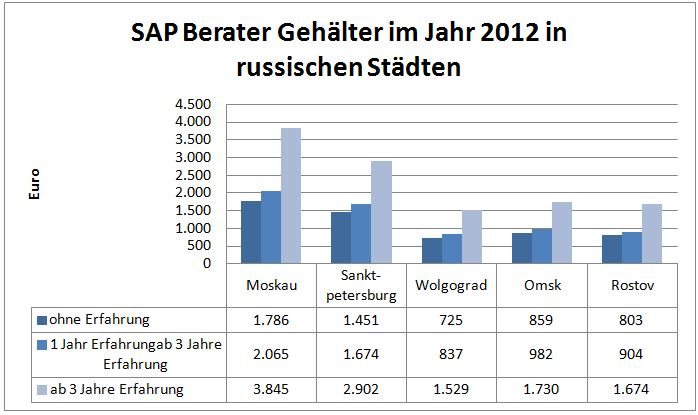
\includegraphics[width=0.7\linewidth]{./images/SAP-Berater_Gehalt_RU}
\caption{SAP-Berater Gehälter in Russland}
\label{fig:SAP-Berater_Gehalt_RU}
\end{figure}
\\
%Quelle:http://www.tadviser.ru/index.php/%D0%A1%D1%82%D0%B0%D1%82%D1%8C%D1%8F:%D0%A0%D1%8B%D0%BD%D0%BE%D0%BA_%D1%82%D1%80%D1%83%D0%B4%D0%B0_%D0%B2_%D0%A0%D0%BE%D1%81%D1%81%D0%B8%D0%B8_(%D0%98%D0%A2_%D0%B8_%D1%82%D0%B5%D0%BB%D0%B5%D0%BA%D0%BE%D0%BC)
	Senior IT-Berater aus Deutschland verdient im Mittel 6.250 € im Monat\cite{GehaltSAPBerDE}. Die deutschen Berater, die nach Ausland geschickt werden, haben noch höheren Gehaltstarif. Der Junior Berater im IT Umfeld ohne Projekterfahrung  verdient in Russland durchschnittlich 1200 € monatlich\cite{GehaltSAPBerRU}. Laut der russischen Arbeitsagentur ``rabota.ru`` steigt die Anfrage auf ERP-Systemen enorm und deswegen steigen auch die Gehälter für Spezialisten in diesem Umfeld. Die Anfänger im IT-Beratungsbereich sind bereit am Anfang der Karriere fast kostenlos zu arbeiten, um Gold werte  Erfahrungen im ERP-Bereich zu sammeln \cite{RusGehRabota}.
	Der deutsche Junior-Berater mit den gleichen Qualifikation und Erfahrung verdient ca. drei mal so viel (3750 €) \cite{GehaltSAPBerDE} als sein russischer Kollege.\\
	\\
	 \newpage
	\textbf{Team und Organisation: Russischer Arbeitskollektiv gegen westlichen Team}\\
	\\
	Das Arbeitskollektiv wurde in der sowjetischen 
	Epoche als das zentrale soziale Handlungsfeld propagiert und die Geschlossenheit der Gruppe ist wichtiger als die Selbstverwirklichung der einzelnen Gruppenmitglieder\cite{ProzessbeglBerRU}.
	Gruppeninterne Konflikte wurden deshalb vermieden oder nicht diskutiert. Der Unterschied zum westlichen Team besteht darin, dass das russische Kollektiv eine dauerhafte Einrichtung mit klar zugewiesene Leitungskompetenzen ist, die vom Vorgesetzten ausgeübt werden, während das Team nur für die Dauer eines bestimmten Projektes eingerichtet wird und sich durch die Gleichberechtigung aller Teammitglieder auszeichnet.
	So ein Kollektiv für Beratungszwecke ist demzufolge nicht flexibel und ist zu stark weisungsgebunden. Die Aufgaben im Kollektiv werden vom Vorgesetzten vorgeschrieben, in unserem Fall von einem Projektleiter oder einem Manager. Solche Führungspersonen sind im IT-Beratungsfall an ein Büro gebunden und sind immer im Büro, während die Berater immer unterwegs bei den Kunden sind. Daher müssen die Entscheidungen immer intuitiv und unabhängig von dem Vorgesetzten getroffen werden. Das ist eine Widerspiegelung von dem Prinzip des russischen Kollektivs. ``Russische Organisationen zeichnen sich durch eine Konzentration von Macht auf die Führungskräfte aus. Ohne den ``Natschalnik`` werden keine Entscheidungen getroffen`` \cite{ProzessbeglBerRU}.
	Verlagerung von Entscheidungen auf die Mitarbeiter wird in Russland selten stattfinden, deswegen werden die Mitarbeiter von der Verantwortung befreit und übernehmen oft nur Anweisungsfunktionen. Für den Beratungsprozess ist diese Tatsache ein großer Minuspunkt, weil die Berater das interdisziplinäres Wissen besitzen und  den vollen Handlungsspielraum in der IT-Beratungsszene brauchen.
	Zu erwähnen wäre noch, dass die jungen Menschen von solcher Stereotypen weiter entfernt sind als die ältere ``sowjetische`` Generation. \\

	\textbf{Personalauswahl und Gesetze}\\
	\\
	 Eine weitere wichtige Besonderheit ist die Personalauswahl. Häufig erfolgt die Auswahl von neuen Mitarbeitern nicht nach Kriterien der fachlichen Kompetenz. Oft werden Arbeitsplätze unter Verwandten und Freunden vergeben. Es existieren fast keine etablierten Mechanismen von Angebot und Nachfrage auf dem Arbeitsmarkt. Vakanzen werden häufig nicht an den fachlich geeignetsten Bewerber vergeben, sondern an ``unseren Mann``(nash celovek).\\
	 Ein weiteres typisches Merkmal für die russische Arbeitskultur ist, dass die Gesetze, Bestimmungen und Regelungen keinen eindeutig verbindlichen Charakter haben. In Abhängigkeit von der Situation und den involvierten Personen, können Regeln oder Gesetze bewusst unberücksichtigt bleiben. Wie sich jedoch diese Abstufung darstellt, ist nicht vorhersagbar. Das liegt auch daran, dass das russische Volk und die russischen Behörde sich einander nicht vertrauen. \cite{ProzessbeglBerRU}.
 
	 \textbf{Arbeitszeit und Urlaub}\\
	 \\
	 Die gesetzliche Wochenarbeitszeit in Russland beträgt 40 Stunden. Doch in meisten Fällen wird diese Grenze total überschritten. Die IT-Spezialisten arbeiten zwischen 10 und 11 Stunden am Tag in einem 5-Tage-Rhythmus \cite{ArbZeitRU}. 
	  Oft wird auch 6-Tage-Woche praktiziert. Die deutschen Berater arbeiten ca. 10 Stunden  im 4 Tage-Rhythmus und sind direkt beim Kunde vor Ort. Am Freitag gibt es entweder Zeit für eigene Weiterbildung im Home-Office oder ein lokales Meeting in der Firma bis nachmittags.
	 In vielen Tarifverträgen in Deutschland beträgt der Jahresurlaub 30 Arbeitstage. In Russland sind es dagegen nur 24 Tage. Der Arbeitstag beginnt bei russischen nicht produzierenden Firmen um 9 oder 10 Uhr \cite{ArbZeitRU}. Wenn ein IT-Berater um 10 Uhr mit seiner Arbeit beginnt, dann ist er um 20-21 Uhr zu hause. Solche Sachen wie Freunde, Familie und Work-Life-Balance stehen nicht direkt im Vordergrund.   \\ \\
	 \textbf{Reisen und Pünktlichkeit}\\
	 \\
	 IT-Berater-Beruf ist eine Tätigkeit, die mit höheren Reisebereitschaft verbunden ist. In Deutschland sind die Berater ganz oft mit Autos unterwegs. Von einem deutschen Großstadt bis zum anderen braucht man beispielsweise 4-5 Stunden. In Russland gibt es 2 grundsätzliche Transportprobleme mit dem Consulting-Hintergrund, die dem Autor auf den ersten Blick erscheinen. Diese sind Staus in Moskau und große Entfernungen zwischen den russischen Städten. Nachfolgend werden diese 2 Probleme näher erläutert. Das Land ist im internationalen Verhältnis sehr groß und weit (es umfasst 11 Zeitzonen).
	 Zwischen Moskau und Nowosibirsk sind es ca 4 Stunden nur Flugzeit und 3 Stunden Zeitunterschied. Wenn ein Berater aus Moskau seinen Arbeitstag am Montag in Nowosibirsk beginnen möchte, muss er schon am Sonntag anreißen. Die Reisen sind erschöpfend und werden von russischen Berater nicht so gern angenommen. Diese stören folglich auch das Work-Life-Balance von IT-Beratern, weil die Reisen direkt ins Privatleben eingreifen und sehr viel zusätzliche Zeit kosten.\\
	 Laut dem russischen Rating "Consulting research" aus 21 größten IT-Consulting-Unternehmen befinden sich 13 Unternehmen in Moskau \cite{RaitConsRU}.
	 Aus 100 größten russischen IT-Unternehmen befinden sich in Moskau 71 Firmen \cite{100BigITConsURU}. 
	 Moskau ist nicht nur ein teuerster Hauptstadt der Welt und ein wirtschaftliches Zentrum des Landes, sondern auch ein strategisches Standort für IT geworden.
	 Mit der Stadtwachstum werden die Staus länger und länger.``Nach Angaben des GPS-Navigationsanbieters TomTom ist Mosaku Nummer eins unter den schlimmsten Stau-Städten der Welt\cite{MoskauStau1}.``
	 Da die Berater öfters unterwegs sind, ist es eine große Anstrengung in Moskau Auto zu fahren. Um von A nach B zu kommen wird ganz oft ein Metro benutzt. 
	 Deswegen ist es in Moskau ``erlaubt`` dem Berater sowie allen Geschäftsleuten ein Viertel bis halbe Stunde zum Meeting oder zum  Kunde zu spät zu kommen. Oft werden Staus als Ausrede, die auch akzeptiert wird, genutzt.\\
	 Allgemein zählt die Pünktlichkeit nicht zu den Stärken von Russen: die Termine werden nicht immer eingehalten, E-Mails werden nicht sofort beantwortet und die Versprechungen sind nicht immer realistisch. Deswegen muss man als Berater diese Verzögerungen mit einplanen \cite{RusKnigge}.\\ \\
	 	 \textbf{Hierarchie und Entscheidungsfindung}\\
	 	 \\
	 Im Teilaspekt Organisation habe ich erwähnt ,dass in russischen Organisationen der Chef oder sogenannte Generaldirektor  allein das Sagen hat. So beschreibt auch der Sergey Frank, dass die Entscheidungskompetenzen in Russland nicht wie gewöhnt nach unten gehen, sondern nur der Geschäftsführer die Entscheidungsbefugnisse hat \cite{RuSFI}.
	 Deswegen kommunizieren die russische IT-Berater oft nur mit dem Geschäftsführer des Unternehmens, was natürlich zur zeitlichen Verzögerungen im Projekt führen kann.\\
	 Gemäß dem ``Russland-Knigge`` \cite{RusKnigge} werden die Hierarchien in Russland nicht eindeutig und nicht klar erkennbar. Die Berater müssen schon vor Beginn der Verhandlungen herausfinden wer das entscheidende Wort hat, damit keine Zeit durch unnötige Gespräche zu verlieren geht.\\
	 Laut dem ``Businessknigge Russland`` sind ``die Flache Hierarchien nicht die Sache der Russen`` \cite{RusKnigge}. 
	 %http://www.hierarchystructure.com/russian-business-hierarchy/
	
	\subsubsection{Japan}
	\textbf{Pünktlichkeit, Kritik und Besonderheit der Kommunikation}\\
	\\
	Im Geschäftsleben sind die Japaner besonders pünktlich. Pünktlich bedeutet in diesem Fall 5 bis 10 Minuten vor einem Termin zu erscheinen. Selbst nur bei 5 Minuten Verspätung müssen Sie an Ihren Geschäftspartner Bescheid geben, dass Sie sich verspäten. \cite{KastensystemInd}. \\
	Die Kritik wird in Japan nicht direkt, sondern ausweichend und über den ``Umweg`` geäußert. Diese Kritikäußerung-Strategie wird auch von ausländischen Geschäftspartner erwartet. Eine Besonderheit in Japan hat die Bedeutung des Wortes ``Ja``: in einem Gespräch reagiert man mit ``Ja`` nicht auf die Zustimmung mit der Sache, sondern auf die Bestätigung des Zuhörers \cite{JPKnigge}. Also schemmen Sie sich in Japan als IT-Berater nicht  ``Ja,Ja`` zu sagen.\\
	\\
	\textbf{Rangordnung und Hierarchie}\\
	\\
	Im japanischen Geschäftsleben spielt die Rangordnung eine wichtige Rolle.
	Beim Essen sitzt die wichtigste Person in der Mitte der Reihe, je größer die Entfernung von ihr, desto geringer der Rang \cite{Business-KniggeFernost}.	
	Beim Meeting wird der Ranghöchste zuerst sprechen. Bei der Begrüßung wird zuerst die Hand nicht der Frau gegeben, wie das in Deutschland üblich ist, sondern dem Ranghöchsten. Wie man den Ranghöchsten bei dem ersten Kontakt ermittelt, ist dem Autor unbekannt.\\
	\\
	\textbf{Arbeitszeit und Urlaub}\\
	\\
	Offiziell gilt in Japan 40-Stunden-Woche, in der Realität sind Angestellten bis 21 oder 23 Uhr im Büro. Wenn jemand eher nach Hause geht als sein Chef, muss bei der nächsten Beförderung mit Konsequenzen rechnen \cite{ArbZeitJP}. Den Arbeitsplatz eher als der Chef zu verlassen, zählt in Japan zu den schlechten Manieren im Geschäftsleben.
	Der Überschrift eines Online-Zeitungsartikels ``Im Japan arbeitet man sich bis zum Tode`` hat sich schon lange als Stereotyp in Japans etabliert. 
	16 Stunden am Tag im Büro, Schlafkammer, Mittagsschläfchen im Zug, unzählige Überstunden gehören zum modernen Arbeitsalltag in Japan. ``Schuld daran haben die Zeitarbeitsagenturen, denn ca. ein Drittel der japanischen Arbeiterschaft besteht aus Zeitarbeitern``, sagt der amerikanische Journalist Jake Adelstein \cite{JPArbeit}. Im Gegensatz zu Deutschland, wo die Überstunden nicht immer bezahlt werden, werden in Japan die Überstunden zur  notwendigen zusätzlichen Geldquelle, ohne diese mancher schwer überleben könnte.
	Es konnten keine konkreten Arbeitszeiten für IT-Berater erhoben werden, jedoch lässt sich auf  Grund der generell erhöhten Arbeitszeiten in Japan auf eine ähnliche Situation im IT-Consulting schließen. 

	In Deutschland genießen die Arbeitnehmer 30 Tage einen bezahlten Urlaub. In den USA beträgt Jahresurlaub rund 2 Wochen. Offiziell sind in Japan im Durchschnitt 17 Freitage gewährt, allerdings werden nur 8 Tage im Krankheitsfall in Anspruch genommen. Da während des Urlaubs keine Lohnfortzahlung stattfindet, muss oft Urlaub unter einer Krankheit ``versteckt`` werden \cite{JPArbeitSozKultur}. Den die Abwesenheit im Krankheitsfall wird vom Unternehmen akzeptiert und eine Lohnfortzahlung wird gezahlt.\\
	\\
		\textbf{Steuer und Lebensstandards}\\
		\\
		Steuern und Sozialabgaben sind in Japan niedriger als in Deutschland. Die japanische Mehrwertsteuer beträgt im Gegensatz zu Deutschland nur 10 \%.
		``Als Arbeitnehmer ist man in Firmen mit mehr als fünf Angestellten durch eine Employee Health Insurance abgesichert``. Jedoch muss man 10 bis 30 Prozent der Behandlungskosten aus eigener Tasche zahlen. Die Arbeitslosenkosten übernimmt der Arbeitgeber \cite{ArbZeitJP}.
		\\Der Lebensstandard im Land der aufgehenden Sonne ist vergleichbar mit dem mitteleuropäischen (sieh die Abb.4.4).
		\begin{figure}[ht]
		\centering
		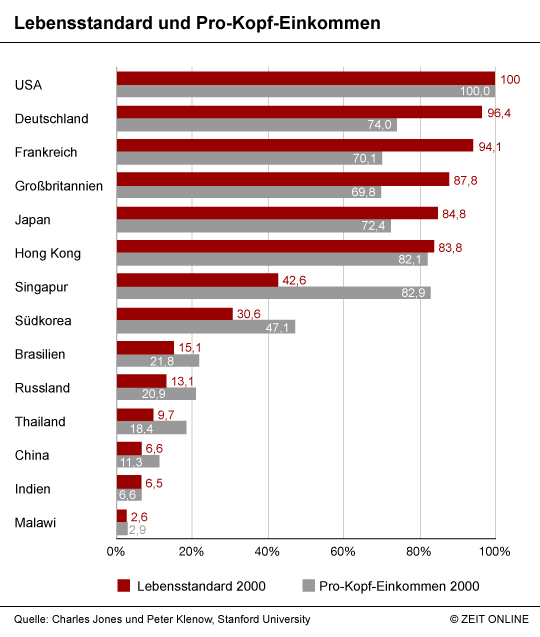
\includegraphics[width=0.7\linewidth]{./images/Lebensstandard-Pro-Kopf-Einkommen}
		\caption{Lebensstandard und Pro-Kopf-Einkommen \cite{LebensStd}}
		\label{fig:LebStdProKEink}
		\end{figure}\\
		Gemäß dem Miroslav Stimac sind die Ausgaben der Grundbedürfnisse in Deutschland höher als in Japan \cite[101]{Stimac2004}.
		Beispielsweise kostet Nahrung in Tokio durchschnittlich 2,36 mal mehr als in Deutschland. Viele japanische Städte leiden an Platznot, dies führt zu hohen Grundstückspreisen sowie Mietpreisen \\cite[105]{Stimac2004}.
		Eine Familie mit 4 Mitgliedern im Großraum Tokio lebt oft in einer 60 qm-Wohnung \cite{ArbZeitJP}.\\	
		Einkommen in Japan hängt von dem  Alter und der Betriebszugehörigkeit
		der Arbeitnehmer ab. Dazu kommt noch der Senioritätsprinzip, der die Gehaltshöhe dem Alter entsprechend definiert. Laut den Angaben  einer Studie der internationalen Personalagentur ``Robert Walters`` verdient ein Projektmanager in der japanischen IT-Branche rund 12 bis 17 Millionen Yen(84.000-119.000 €).
		Systemadministratoren verdienen ca 9 bis 14 Millionen Yen(63.000-98.000 €) \cite{EinkommenJP}.
		Diese Gehälter sind sehr beeindruckend. Die Daten zu den IT-Berater-Gehälter könnte ich nicht gefunden, meiner Meinung nach müssen diese nicht kleiner als die Gehälter von Systemadministratoren sein. \\
			\textbf{Gruppe}\\
			\\
		Die Bedeutung der Gruppe sowie ihr Erfolg laut Michael Gehle orientiert sich nicht auf die individuellen Ziele der	einzelnen Gruppenmitglieder, sondern auf ein gemeinsames Erfolg der Gruppe. Altruistisches Verhalten ist in japanischer Gesellschaft ausgeprägter als in Europa. Das Wohl der Einzelnen ist vom Wohl seiner Kollegen abhängig. Mit anderen Worten bedeutet dass, die erfolgreiche Zusammenarbeit der Gruppe eng an die interne Zusammenarbeit der Gruppenmitglieder angebunden  ist. Damit wird auch die Gruppe,  ähnlich wie eine Familie, die Schutzfunktion übernehmen, denn nicht nur das Erfolg des gesamten Projektes sondern auch das Risiko an die Gruppenzugehörigen zu verteilen ist \cite[233]{3LaenderVergl}.\\ \\
		\textbf{Entscheidungsfindung} \\ \\
		Im Gegensatz zu Russland werden die Entscheidungsbefugnisse auch an die untere Hierarchieebene delegiert. Damit werden auch die hohe Managementanforderungen  an die normalen Mitarbeitern gestellt \cite[233]{3LaenderVergl}.\\
		Die Japaner haben ewig lange Entscheidungswege. Die Entscheidung wird nach top-down-Methode vom Chef angestoßen, dann verläuft die Akzeptanz der Entscheidung durch eine Organisationsspirale bis jeder Mitarbeiter diese Entscheidung wahrgenommen hat. In Deutschland wird die Entscheidungen eher nach Formalismus getroffen. Innerhalb des Teams gilt eine Gleichberechtigung und der Chef hat eine Rolle des Moderators. Falls während des Projektes die Probleme aufgetreten sind, wird in Japan der Projektmanager nicht kritisiert und Schuld wird an alle Projektmitglieder verteilt. In Deutschland dagegen trägt der Projektleiter ganz oft die ganze Verantwortung für Misserfolg des Projektes.
%ab hier Korrektur
	\subsubsection{USA}
	\textbf{Gruppe}\\
	\\
	In USA sowie in Deutschland hängt der Erfolg sowie die Karriere des einzelnen Gruppenmitglieder nicht so stark vom Gruppenerfolg wie in Japan ab. Zwar haben die westlichen Gruppenmitglieder auch ein gemeinsames Ziel und arbeiten kollaborativ, trotzdem durch die Aufgaben- und Verantwortungsverteilung besitzt die Gruppe in USA eine untergeordnete Rolle. Laut dem Michael Gehle orientiert sich die  Karriere und Qualifizierungsmaßnahmen an einzelnen Mitarbeitern, deswegen richtet sich auch deren Verhalten eher nach individuellen und nicht nach kollektiven Zielen \cite[233]{3LaenderVergl}. 
	Teamkollegen werden in USA sowie in westlichen Ländern nicht selten als Konkurrenten angesehen, weil die Entlohnung sowie Kontrolle der Mitarbeiter an den individuellen Leistungen angehängt werden. In Japan wird dagegen durch den Sozialisationsprozess die Gruppenmitlieder eher als Familienmitglieder angesehen.\\
	 \\
		\textbf{Arbeitszeit und Urlaub}\\
		\\
	Arbeitszeit in den USA beträgt in der Regal 40 Stunden pro Woche. 
	Ein Drittel aller Amerikaner arbeiten länger als 40 Stunden pro Woche.
	Laut einer UN-Studie arbeiten US-Angestellte im Durchschnitt etwa 500 Stunden mehr als deutsche Arbeitnehmer \cite{ArbeitsumgUSA}! Die Meisten Amerikaner haben nur 10 bezahlten Arbeitstage \cite{InfoUSArbVertr}. 
	\\
	\\	\textbf{Besonderheiten in Arbeitsgesetzen}\\
		\\
		Die Lohnfortzahlung im Krankheitsfall beträgt in USA nur 7 Tage pro Jahr. 
		Mitarbeiter im IT Bereich haben keinen Anspruch auf Überstundenausgleich, man kann aber inoffiziell ein zusätzlichen Tag in der Woche frei nehmen um die Überstunden auszugleichen. Als Überstundenausgleich dient auch am Ende des Jahres ein finanzieller Bonus \cite{InfoUSArbVertr}.
		Solche Vereinbarungen sind aber nicht gesetzlich geregelt und müssen mündlich ausgemacht werden.\\
		Die Kündigungsfrist beträgt, sowohl für Arbeitgeber als auch für 
		Arbeitnehmer, zwei Wochen. Aufgrund der kurzen Kündigungsfrist gibt es in den USA keine Probezeit.\\
		Im ersten Arbeitsjahr gibt es in USA kein Anspruch auf Urlaub \cite{USA_Tipps}.
		\\ \\
	\textbf{Gehalt von IT-Berater}\\
		\\
		Laut der Firma ``indeed`` beträgt ein Jahresgehalt des IT-Beraters (Technical Consultant`s in USA) rund 86.000 \$(sieh Abb. 4.5).
		\begin{figure}[ht]
				\centering
				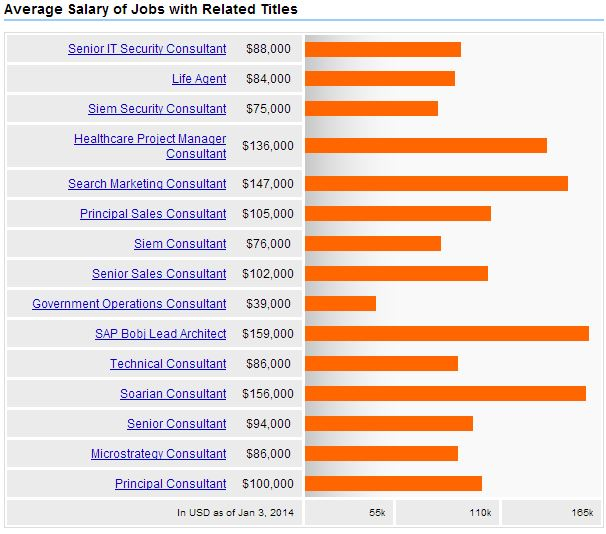
\includegraphics[width=0.7\linewidth]{./images/Techn_Cons_Sal}
				\caption{Jahresgehalt von IT-Consultants in USA}
				\label{fig:TechConsSal}
				\end{figure}\\
				%Wo ist Quelle???
		``Ein europäisches Gehalt in EUR ist ungefähr 1:1 vergleichbar mit einem 
		amerikanischen Gehalt in USD. Es wäre nicht richtig, den offiziellen Umrechnungskurs anzusetzen, da die Lebenshaltungskosten in USD in den USA mit den Lebenshaltungskosten in EUR in Europa vergleichbar sind	`` \cite{InfoUSArbVertr}. In der IT-Branche wird oft ein Provision angeboten, die von erfolgreichen 
		Projekten abhängt. Das Gehalt wird immer in zwei Raten ausbezahlt, in der Regel am 15. und am letzten Tag des Monats.\\ \\
	\textbf{Hierarchie} \\ \\
	Gemäß dem US-Internetportal ``hierarchystructure.com`` \cite{HierarchieUSA} gehört die US- Geschäftshierarchie zu den erfolgreichsten Geschäftshierarchien der Welt und wird von vielen Ländern als Vorbild genommen, um das wirtschaftliche Wachstum zu erzielen. Geschäftsstruktur und Hierarchie einer Organisation werden mit dem Zweck das Gruppenziel zu erreichen aufgebaut, wobei jeder einzelne Mitglied der Organisation unterstützt wird. Dabei werden die Positionen, Aufgaben und zugehörigen Mitarbeiterrollen klar definiert.
\begin{figure}[ht]
\centering
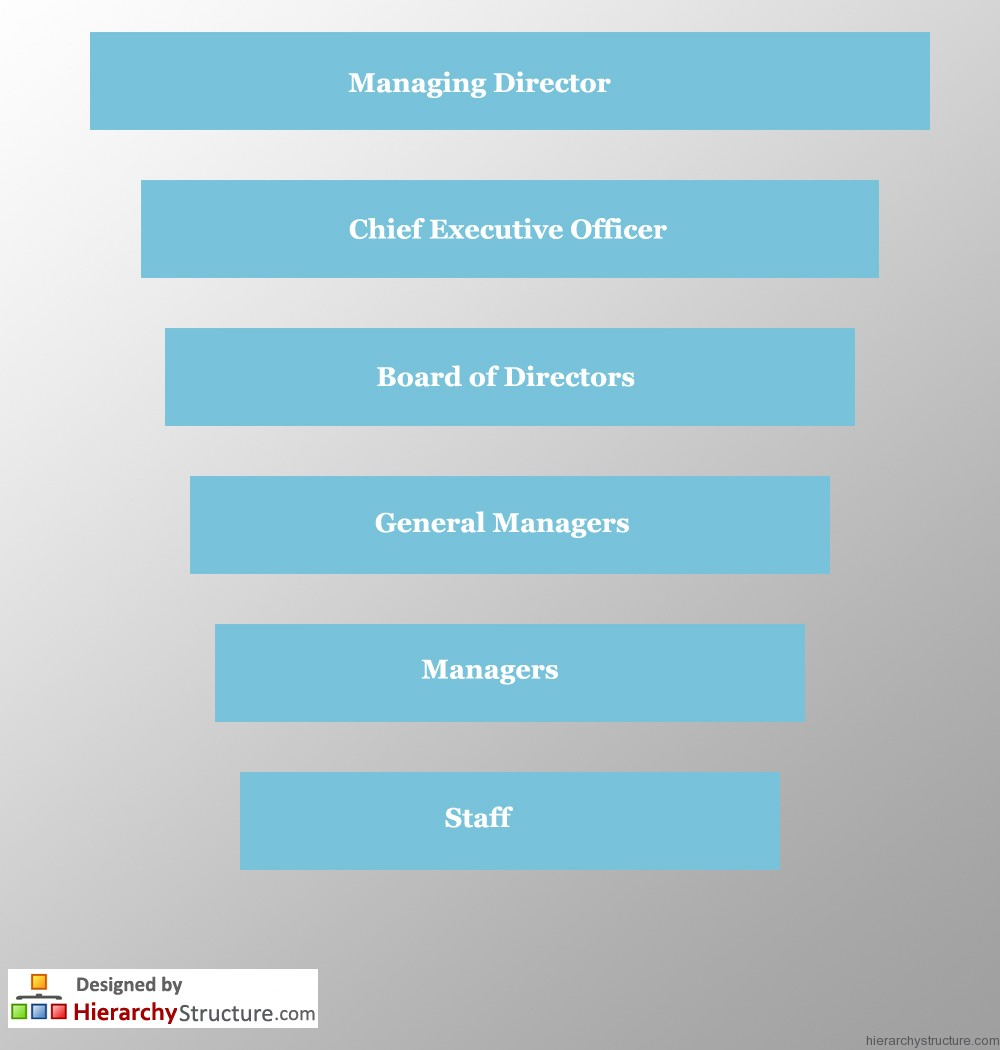
\includegraphics[width=0.7\linewidth]{./images/USA-Business-Hierarchy}
\caption{Geschäftshierarchie USA \cite{HierarchieUSA}}
\label{fig:USA-Business-Hierarchy}
\end{figure}


	\subsubsection{Deutschland}
	In allen beschriebenen Ländern unterscheidet sich erheblich der Formalisierungsgrad der Arbeitskultur. In Deutschland wird das Verhaltenswesen und Standards der Arbeitskultur sehr formalisiert in Form von gesetzlichen Vorschriften definiert. In Japan weist die Arbeitskultur auch einen hohen Formalisierungsgrad auf. Das hat nicht mit gesetzlichen Regelungen wie in Deutschland, sondern eher mit traditionellen Verhaltensweisen zu tun \cite[236]{3LaenderVergl}.
	%Quelle:Michael Gehle, Telearbeit: ein Drei-Länder-Vergleich S. 237->Tabelle!!!!!!!!!!!!
	%1)Teilaspekte umbennenen
	%2)Deutschland
	%3)Indien
	\subsubsection{Indien}
	